%%%%%%%%%%%%%%%%%%%%%%%%%%%%%%%%
%
% 6 sept 2013 [Jan]: lay-out verbeterd, kommagetallen, figuur iets verkleind, foutjes
%
%%%%%%%%%%%%%%%%%%%%%%%%%%%%%%%%%
\chapter{Eerstegraadsfuncties}
\label{chap:eerstegraadsfuncties}
\begin{quote}
     \textit{{\small `En hoeveel uur les hadden jullie per dag?' zei
     Alice, die vlug van onderwerp wilde veranderen.}}

     \textit{{\small `De eerste dag tien uur,' zei de Nepschildpad,
     `de volgende negen enzovoort.'}}

     \textit{{\small `Wat een raar lesrooster!' riep Alice uit.}}

     \textit{{\small `Zo lesten we onze dorst naar kennis steeds
     sneller,' merkte de Griffioen op, `vandaar de uitdrukking ''lest
     best''.'}}

     \textit{{\small Dat was volkomen nieuw voor Alice en ze dacht er
     even over na voordat ze haar volgende opmerking maakte. `Dus
     hadden jullie de elfde dag vrij?'}}

     \textit{{\small `Reken maar,' zei de Nepschildpad.}}

     \textit{{\small `En wat deden jullie met de twaalfde dag?' vroeg
     Alice gretig verder.}}

          Uit `Alice in Wonderland' -- Lewis Carroll
\end{quote}


\newpage
\noindent Veel verbanden tussen grootheden (snelheid, prijs, massa, lengte, aantal \ldots) kunnen voorgesteld worden door een veeltermfunctie van de eerste graad, kortweg \emph{eerstegraadsfunctie}\index{eerstegraadsfunctie}\footnote{Een veelterm van de eerste graad in de veranderlijke $x$ heeft de vorm $a+bx$. Er staat enkel een $x$ (tot de eerste macht) en dus spreken we over `\ldots van de eerste graad'.}. De grafiek hiervan is een rechte. Verder in de cursus maken we geregeld gebruik van eerstegraadsfuncties en rechten (bvb. lineaire programmatie, lineaire groei, rekenkundige rijen). We verwachten dus dat je vlot kan werken met dit type functie. Deze leerstof zag je reeds in het secundair, maar waarschijnlijk kan een herhaling geen kwaad?

\section{Hoeveel kost een taxirit?}\label{sec:taxirit}
Je plant een uitstapje naar Brussel. Alle verplaatsingen in Brussel zelf doe je met een taxi. 
 \begin{figure}[htbp]
      \centering
     \includegraphics[width=\textwidth]{figuren/eerstegraadsfuncties/taxi.jpg}
     \caption{Nieuwe zwartgele Brusselse taxi}
     \label{fig:taxi}
 \end{figure}
Het zou fijn zijn om op voorhand een schatting van de kostprijs te kunnen maken. Op de site van mobielbrussel\footnote{\url{http://www.mobielbrussel.irisnet.be/articles/taxi/hoeveel-kost-een-taxi}} vind je volgende informatie:
\begin{itemize}
\item Instapgeld: \euros{2,40}
\item Tarief I (in de 19 gemeenten van het Brussels Hoofdstedelijk Gewest): \euros{1,80} per km.
\item Tarief II (buiten de 19 gemeenten): \euros{2,70} per km.
\item Wachtvergoeding: \euros{30} per uur.
\item Tussen 22 en 6 uur wordt een forfaitaire meerprijs van \euros{2,00} gevraagd.
\end{itemize}
Hoeveel kost een ritje van 15 km in het centrum om middernacht?  Hoever geraak je 's nachts in het centrum met \euros{20}? 

Om deze vragen te beantwoorden stellen we een \emph{wiskundig model} op. In dit geval gaat het om een eenvoudig model. Het verband tussen de afstand en de kostprijs kan beschreven worden door een lineair model. De bijbehorende functie is een veeltermfunctie van de eerste graad, kortweg `eerstegraadsfunctie' genoemd.

In dit model houden we geen rekening met opstoppingen (en is er dus geen wachtvergoeding) en gaan we uit van een teller die continu doorloopt en per meter registreert (en dus niet per km pas verspringt). Als je nu luidkeels protesteert en het niet eens bent met deze veronderstellingen, heb je natuurlijk groot gelijk. Een taximeter gaat inderdaad met sprongetjes vooruit! We komen hierop in \cref{sec:taxisprong} op pagina~\pageref{sec:taxisprong} terug en bekijken hoe we het model dan kunnen aanpassen. 

\section{Op zoek naar de functie}
In deze sectie gaan we op zoek naar een wiskundig model dat ons de prijs kan geven voor een bepaalde afstand in het centrum 's nachts.
Uit het algemeen hoofdstuk over functies weet je nog dat er verschillende manieren zijn om een functie voor te stellen:
\begin{itemize}
\item een tabel met getallen en bijhorende functiewaarden;
\item een grafiek;
\item een wiskundig voorschrift.
\end{itemize}

\subsection{Enkele functiewaarden berekenen}
Meestal is het een goed idee om te beginnen met enkele \emph{concrete afstanden} de kostprijs te noteren/berekenen en de gevonden waarden te noteren in een tabel. Om alles wat korter te noteren voeren we enkele notaties in. De afstand in km noemen we $x$. Voor de kostprijs in \euro \ gebruiken we $P$. Aangezien er bij elke afstand $x$ juist één kostprijs $P$ hoort is dit verband zeker een functie en mogen we $P(x)$ schrijven.

Gewoon instappen in een taxi (en 0 km rijden) kost op zich al geld. Je betaalt \euros{4,40} aan instapgeld en het nachtforfait. Wiskundig noteren we $P(0)=4,40$.

Als je 1 km rijdt komt er \euros{1,66} bij. Het totale bedrag voor een rit van 1 km is $P(1)=4,40+1,66=6,06$. Nog een km verder is er terug hetzelfde bedrag bijgekomen en wordt de totale kostprijs $P(2)=P(1)+1,66=7,72$. Deze berekening een aantal keer herhalen levert \cref{tbl:taxi}

\begin{table}[htbp]
    \centering
    \caption{Prijs van een taxirit i.f.v. de afstand}
    \begin{tabular}{SSp{2cm}SS}
    \toprule
    {Afstand} & {Kostprijs} & & {Afstand} & {Kostprijs} \\
    \midrule
0 & 4,40 & & 9 & 19,34 \\
1 & 6,06  & & 10 & 21 \\
2 & 7,72 & & 11 & 22,66 \\
3 & 9,38  & & 12 & 24,32 \\
4 & 11,04 & & 13 & 25,98 \\
5 & 12,7 & &14 & 27,64 \\
6 & 14,36 & & 15 & 29,3 \\
7 & 16,02 & & 16 & 30,96 \\
8 & 17,68  & & & \\
    \bottomrule
     \end{tabular}
    \label{tbl:taxi}
\end{table}

We hadden hierboven twee vragen: hoeveel kost een nachtelijke rit van 15 km en hoever geraak je met \euros{20}?
De eerste vraag is eenvoudig op te lossen met de tabel: je zoekt de afstand 15 op in de kolom `Afstand' en
leest op dezelfde rij de prijs af in de `Kostprijs' kolom, nl.\ \euros{29,30}.

De tweede vraag is iets moeilijker. Hoever geraak je met \euros{20}? Hiervoor moeten
we in de prijskolom 20 opzoeken, maar dat staat er niet tussen.
Met behulp van deze tabel kunnen we wel besluiten dat we ergens tussen 9 en \SI{10}{\km} halen. 

\subsection{Een grafische voorstelling}
\label{subsec:grafischeVoorstelling}
We zetten de punten uit \cref{tbl:taxi} in een grafiek.
\emph{Denk even na over de grootte van de assen vooraleer je een figuur maakt.}
Hier lijkt een $x$-as tot 16 en een $y$-as tot 31 aangewezen. Alle punten uit de tabel liggen op \cref{fig:taxir} op \'e\'en rechte.
\begin{figure}[htbp]
    \centering
\begin{tikzpicture}[x=0.5cm,y=0.25cm]
\draw[->] (-1,0) -- (17,0) node[right] {$x$};
\draw[->] (0,-1) -- (0,32) node[above] {$P$};
\foreach \x in {1,2,4,...,15,16}
	\draw[shift={(\x,0)}] (0pt,2pt) -- (0pt,-2pt) node[below] {\footnotesize $\x$};
\foreach \y in {5,10,...,30}
	\draw[shift={(0,\y)},color=black] (2pt,0pt) -- (-2pt,0pt) node[left] {\footnotesize $\y$};
\draw[thick](0,4.5) -- (16,30.96);
\node [below left] at (0,0) {\footnotesize 0};
\filldraw [red] (15,29.3) circle (2pt);
\filldraw [red] (3,9.38) circle (2pt) node[below right] {(3;9,38)};
\filldraw [red] (1,6.06) circle (2pt) node[below right] {(1;6,06)};
\filldraw [red] (8,17.68) circle (2pt) node[below right] {(8;17,68)};
\draw[dashed,-latex](15,0) -- (15,29.3);
\draw[dashed, -latex](15,29.3) -- (0,29.3);
\draw[dashdotted,-latex](0,20) -- (9.397,20);
\draw[dashdotted, -latex](9.397,20) -- (9.397,0);
\end{tikzpicture}
\caption{Prijs $P(x)$ van een taxirit i.f.v. de afstand $x$}
    \label{fig:taxir}
\end{figure}

We kunnen beide vragen nu ook \emph{grafisch} oplossen. Hoeveel kost een rit van 15 km? Teken een verticale (streepjeslijn) bij $x=15$. Deze verticale snijdt de rechte. Door het snijpunt teken je een horizontale. Die snijdt de verticale $P$-as net onder 30. De juiste waarde is op deze figuur niet af te lezen, maar dat is \emph{meestal ook niet de bedoeling van een grafische voorstelling}.

Omgekeerd vroegen we ons af hoever we geraakten met \euros{20}? Vertrek nu van 20 op de $P$-as met een horizontale rechte (punt-streepjeslijn). Door het snijpunt met de prijsrechte komt een verticale rechte. Die snijdt de $x$-as ergens tussen 9 en 10. Opnieuw is de exacte waarde niet af te lezen op de grafiek.



\subsection{Een formule}
Om exacte waarden te berekenen is een voorschrift, een formule vaak de aangewezen voorstellingsvorm voor een functie. We redeneren als volgt: per extra km komt er \euros{1,66} bij. Dit geeft volgende berekeningen:
\begin{align*}
P(0)&=4,40\\
P(1)&=P(0)+1,66=4,40+1,66=6,06\\
P(\mathbf{2})&=P(1)+1,66=4,40+\mathbf{2}\cdot 1,66=7,72\\
P(\mathbf{3})&=P(2)+1,66=4,40+\mathbf{3}\cdot 1,66= 9,38\\
\ldots \ &=\ \ldots \\
P(x)&=4,40+x\cdot 1,66
\end{align*}
Formule~\ref{eq:taxi} geeft bijgevolg het verband tussen de afstand $x$ en de kostprijs $P$. Het is een veeltermfunctie van de eerste graad, kortweg `eerstegraadsfunctie' of `lineaire functie' genoemd.
\begin{equation}\label{eq:taxi}
P(x)=1,66\cdot x + 4,40
\end{equation}
Deze formule laat ons nu toe om het antwoord op bovenstaande vragen via rekenwerk op te lossen. Hoeveel kost een rit van 15 km? Vul $x=15$ in formule~\eqref{eq:taxi} in:
\[
P(15)=1,66\cdot 15 + 4,40=29,30.
\]
Deze rit kost dus \euros{29,30}.

De omgekeerde vraag vergt iets meer werk. Hoever geraak je met \euros{20}? Merk op dat we nu de prijs $P$ krijgen en dat men de afstand $x$ vraagt. De prijs invullen levert een vergelijking in de onbekende $x$, die je oplost volgens de regels van de algebra:
\begin{align*}
20&=1,66\cdot x + 4,40\\
\Leftrightarrow 20-4,40&=1,66 \cdot x\\
\Leftrightarrow \dfrac{15,60}{1,66}&=x\\
\Leftrightarrow 9,3976 &= x
\end{align*}
Met \euros{20} geraken we dus 9,4 km (afgerond) ver.

\section{Richtingscoëfficiënt}
\subsection{Inleiding}
We hernemen \cref{fig:taxir} in \cref{fig:taxiredetail}.
\begin{figure}[htbp]
    \centering
\begin{tikzpicture}[x=1.8cm,y=0.8cm]
\draw[->] (-0.5,0) -- (4.5,0) node[right] {$x$};
\draw[->] (0,-0.5) -- (0,11.5) node[above] {$P$};
\foreach \x in {1,...,4}
	\draw[shift={(\x,0)}] (0pt,2pt) -- (0pt,-2pt) node[below] {\footnotesize $\x$};
\foreach \y in {1,...,11}
	\draw[shift={(0,\y)},color=black] (2pt,0pt) -- (-2pt,0pt) node[left] {\footnotesize $\y$};
\draw[thick](0,4.4) -- (4.1,11.206);
\node [below left] at (0,0) {\footnotesize 0};
\filldraw [red] (0,4.4) circle (2pt) ;
\filldraw [red] (3,9.38) circle (2pt) ;
\filldraw [red] (1,6.06) circle (2pt) ;
\filldraw [red] (2,7.72) circle (2pt) ;
\filldraw [red] (4,11.04) circle (2pt) ;
\draw[thick,donkergroen,-latex](0,4.4) -- (1,4.4) node[midway,above] {$+1$};
\draw[thick,blue,-latex](1,4.4) -- (1,6.06) node[midway,right] {$+1,66$};
\draw[thick,donkergroen,-latex](1,6.06) -- (2,6.06) node[midway,above] {$+1$};
\draw[thick,blue,-latex](2,6.06) -- (2,7.72) node[midway,right] {$+1,66$};
\draw[thick,donkergroen,-latex](2,7.72) -- (3,7.72) node[midway,above] {$+1$};
\draw[thick,blue,-latex](3,7.72) -- (3,9.38) node[midway,right] {$+1,66$};
\end{tikzpicture}
\caption{Rechte heeft rico 1,66}
    \label{fig:taxiredetail}
\end{figure}
\Cref{fig:taxiredetail} toont het belang van het getal 1,66. Per gereden km komt er \euros{1,66} bij de prijs bij. Als je op de grafiek in een punt van de rechte vertrekt en je tekent een horizontale rechte met lengte 1, dan is de lengte van het lijnstukje dat je verticaal naar boven moet gaan om terug op de rechte uit te komen gelijk aan 1,66. Deze afstand 1,66 wordt de \emph{richtingscoëfficiënt}\index{richtingsco\"effici\"ent}\index{rico} van de rechte genoemd (kortweg: \emph{rico}). 

\subsection{Berekening}
Gegeven een rechte door twee gegeven punten $(x_1, y_1)$ en $(x_2,y_2)$. De rico is dan
\begin{equation}\label{eq:rico}
\text{rico}=\dfrac{\text{\textcolor{blue}{verticale toename}}}{\text{\textcolor{donkergroen}{horizontale toename}}}=\dfrac{\textcolor{blue}{y_2-y_1}}{\textcolor{donkergroen}{x_2-x_1}}
\end{equation}
\begin{figure}[htbp]
    \centering
\begin{tikzpicture}[x=1cm,y=1cm]
\draw[->] (-0.5,0) -- (3.5,0) node[right] {$x$};
\draw[->] (0,-0.5) -- (0,4) node[above] {$y$};
\draw[shift={(1,0)}] (0pt,2pt) -- (0pt,-2pt) node[below] {\footnotesize $x_1$};
\draw[shift={(3,0)}] (0pt,2pt) -- (0pt,-2pt) node[below] {\footnotesize $x_2$};
	\draw[shift={(0,2)},color=black] (2pt,0pt) -- (-2pt,0pt) node[left] {\footnotesize $y_1$};
	\draw[shift={(0,3)},color=black] (2pt,0pt) -- (-2pt,0pt) node[left] {\footnotesize $y_2$};
\draw[thick](0.5,1.75) -- (3.5,3.25);
\node [below left] at (0,0) {\footnotesize 0};
\draw[dashed] (0,2) -| (1,0);
\draw[dashed] (0,3) -| (3,0);
\filldraw [red] (1,2) circle (2pt) ;
\filldraw [red] (3,3) circle (2pt) ;
\draw[thick,donkergroen,-latex](1,2) -- (3,2) node[midway,below] {$x_2-x_1$};
\draw[thick,blue,-latex](3,2) -- (3,3) node[midway,right] {$y_2-y_1$};
\end{tikzpicture}
\caption{Rico van rechte door twee punten}
    \label{fig:defrico}
\end{figure}
De rico van een rechte is dus volgens formule~\eqref{eq:rico} een breuk. De aandachtige lezer herinnert zich nog uit het secundair dat de noemer van een breuk nooit gelijk aan 0 mag worden. Dat is het geval als $x_2=x_1$, dus als beide punten op een verticale rechte liggen. We besluiten bijgevolg: \emph{de rico van een verticale rechte is niet gedefinieerd}.

\subsection{Stijgen en dalen}
De rico is een maat voor de toename van een grootheid als een andere grootheid toeneemt. Als ik 1 km met een taxi verder rijd, komt er \euros{1,66} bij de rekening bij. Een ritje buiten het centrum van Brussel kost \euros{2,70} per km zoals we zagen. De rechte die de prijs van zo'n taxirit weergeeft in functie van de afstand heeft dus een grotere rico. 

We kunnen voor de rico drie gevallen onderscheiden.

\subsubsection{Rico groter dan 0}
Een positieve rico komt overeen met een stijgende rechte. Hoe groter de rico, des te steiler stijgt de rechte. We spreken dan over een functie die een \emph{lineaire toename} kent.

\subsubsection{Rico kleiner dan 0}
Als de rico negatief is, daalt de functie. Het gaat hier dan om een functie die afneemt als de waarden op de horizontale as groter worden: \emph{lineaire afname}. 

\subsubsection{Rico gelijk aan 0}
De rico wordt 0 als $y_2-y_1=0$, dus als $y_2=y_1$. De twee punten liggen dan op een horizontale rechte. Er is geen toe- of afname meer. De functiewaarde is een \emph{constante} en hangt dus niet af van de waarde op de horizontale as. Alsof je in een taxi stapt die een vaste prijs heeft, hoe ver de rit ook is.

\section{Functievoorschrift}
\label{sec:functievoorschrift}
\subsection{Algemeen}
Algemeen ziet een lineaire functie er uit als
\begin{equation}\label{eq:linfunc}
f(x)=mx+q
\end{equation}
De coëfficiënt van $x$ (het getal $m$) vertelt iets over het stijgen en dalen van de rechte: de rico. Het getal $q$ is de $y$-waarde waarbij de rechte de verticale as snijdt. Immers, als we $x=0$ stellen in vergelijking~\eqref{eq:linfunc}:
\begin{align*}
f(0)&=m\cdot 0 + q\\
&= q
\end{align*}
Het getal $q$ is dus de functiewaarde in 0. Men noemt $q$ daarom soms ook de \emph{startwaarde}\index{startwaarde} van de functie, zeker als de veranderlijke op de horizontale as de tijd is.

We zullen in het vervolg van deze tekst de begrippen \emph{functievoorschrift} en \emph{vergelijking} door elkaar gebruiken. Het verschil is ondermeer dit: $f(x)=2x+3$ is het voorschrift van een eerstegraadsfunctie (of lineaire functie). Als we $f(x)$ vervangen door $y$ spreken we liever van een vergelijking van de rechte: $y=2x+3$. Vergelijkingen van rechten kunnen we bovendien algebraïsch aanpassen, bvb. $y-2x=3$ of $2x-y+3=0$ stelt telkens dezelfde rechte voor.

\subsection{Rechtevenredig verband}
Als in vergelijking~\eqref{eq:linfunc} de waarde van $q$ gelijk gesteld wordt aan 0, gaat de rechte door de oorsprong. De rechte krijgt dan als vergelijking $f(x)=mx$. We spreken dan over een \emph{rechtevenredig verband}\index{recht evenredig}.

Deze speciale eerstegraadsfunctie komt veel voor, bvb. 
\begin{itemize}
\item Bellen met een oplaadkaart: niet bellen kost \euros{0}. Vijf minuten bellen kost 5 keer zoveel als 1 minuut bellen. Het verband tussen de prijs en het aantal minuten is rechtevenredig.
\item Gehakt kopen bij een beenhouwer: als je \SI{0}{\gram} koopt kost het \euros{0}. Wie \SI{800}{\gram} gehakt koopt, betaalt 8 keer zoveel als iemand die \SI{100}{\gram} koopt.  Het verband tussen de prijs en de massa is rechtevenredig.
\end{itemize}

\section{De vergelijking van een rechte opstellen}
\Cref{fig:rechtevgl} toont een rechte. Hoe vind je het bijpassende functievoorschrift? We overlopen een aantal methodes die je in het derde jaar secundair in detail inoefende.
\begin{figure}[htbp]
    \centering
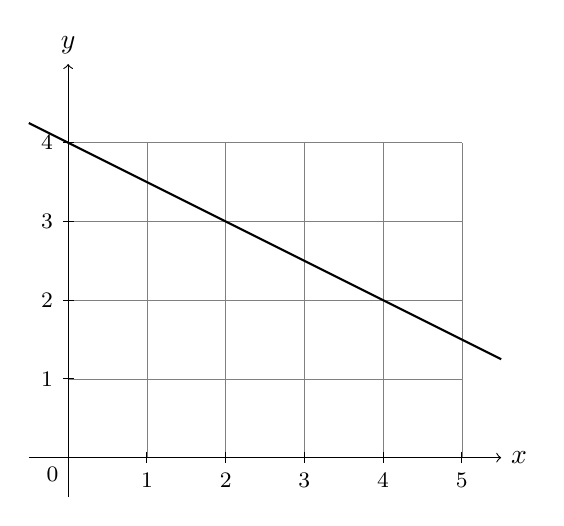
\begin{tikzpicture}[x=1cm,y=1cm]
\draw[help lines] (0,0) grid (5,4);
\draw[->] (-0.5,0) -- (5.5,0) node[right] {$x$};
\draw[->] (0,-0.5) -- (0,5) node[above] {$y$};
\foreach \x in {1,...,5}
	\draw[shift={(\x,0)}] (0pt,2pt) -- (0pt,-2pt) node[below] {\footnotesize $\x$};
\foreach \y in {1,...,4}
	\draw[shift={(0,\y)},color=black] (2pt,0pt) -- (-2pt,0pt) node[left] {\footnotesize $\y$};
\draw[thick](-0.5,4.25) -- (5.5,1.25);
\node [below left] at (0,0) {\footnotesize 0};

\end{tikzpicture}
\caption{Wat is de vergelijking van deze rechte?}
    \label{fig:rechtevgl}
\end{figure}

\subsection{Met snijpunt y-as en rico}
De rechte van \cref{fig:rechtevgl} snijdt de verticale as in het punt $(0,4)$ en dus is in vgl~\eqref{eq:linfunc} $q=4$. Met een kleine hulpconstructie (\cref{fig:rechtevgl2}) en formule~\eqref{eq:rico} vinden we als rico $m=\frac{-1}{2}$ (negatief want de rechte daalt). De gevraagde vergelijking wordt dus
\[
y=\frac{-1}{2}x+4
\]
en het functievoorschrift voor deze eerstegraadsfunctie is dus
\[
f(x)=\frac{-1}{2}x+4.
\]
\begin{figure}[htbp]
    \centering
\begin{tikzpicture}[x=1cm,y=1cm]
\draw[help lines] (0,0) grid (5,4);
\draw[->] (-0.5,0) -- (5.5,0) node[right] {$x$};
\draw[->] (0,-0.5) -- (0,5) node[above] {$y$};
\foreach \x in {1,...,5}
	\draw[shift={(\x,0)}] (0pt,2pt) -- (0pt,-2pt) node[below] {\footnotesize $\x$};
\foreach \y in {1,...,4}
	\draw[shift={(0,\y)},color=black] (2pt,0pt) -- (-2pt,0pt) node[left] {\footnotesize $\y$};
\draw[thick](-0.5,4.25) -- (5.5,1.25);
\node [below left] at (0,0) {\footnotesize 0};
\filldraw [red] (0,4) circle (2pt) ;
\filldraw [red] (2,3) circle (2pt) ;
\draw[thick,donkergroen,-latex](0,4) -- (2,4) node[midway,above] {$+2$};
\draw[thick,blue,-latex](2,4) -- (2,3) node[midway,right] {$-1$};
\end{tikzpicture}
\caption{Rico grafisch bepalen}
    \label{fig:rechtevgl2}
\end{figure}

\subsection{Eén punt en rico gegeven}
Stel dat je gegeven krijgt dat de rechte door het punt $(2,3)$ gaat en dat de rico gelijk is aan $-0,5$. Er zijn twee manieren om de vergelijking van deze rechte te vinden.

\subsubsection{Manier 1: punt invullen in algemene vergelijking}
Als de rechte een rico $-0,5$ heeft, dan heeft ze de algemene vorm $y=-0,5x+q$. Het snijpunt met de verticale as, $q$, kennen we niet. Het punt $(2,3)$ ligt op de rechte. \emph{`Liggen op'} betekent: \emph{`je mag dit punt invullen in de vergelijking'}. Invullen komt neer op $x$ vervangen door 2 en $y$ door 3. We bekomen 
\begin{align*}
3&=-0,5\cdot 2 + q\\
\Leftrightarrow 3&=-1+q\\
\Leftrightarrow 4&=q
\end{align*}
De gezochte vergelijking wordt dus: $y=-0,5x+4$.

\subsubsection{Manier 2: algemene formule gebruiken}
De vergelijking van een rechte door een gegeven punt $(x_1,y_1)$ met gegeven rico $m$ wordt gegeven door
\begin{equation}\label{eq:puntrico}
y-y_1=m(x-x_1).
\end{equation}
Formule~\eqref{eq:puntrico} uitrekenen voor het punt $(2,3)$ en rico $-0,5$ levert
\begin{align*}
y-3&=-0,5(x-2)\\
\Leftrightarrow y-3&=-0,5x + 1\\
\Leftrightarrow y&=-0,5x+4
\end{align*}

\subsection{Twee punten gegeven}
Dit kunnen we als een speciaal geval van formule~\eqref{eq:puntrico} zien. De vergelijking van een rechte door twee gegeven punten $(x_1,y_1)$ en $(x_2,y_2)$ wordt gegeven door
\begin{equation}\label{eq:puntpunt}
y-y_1=m(x-x_1) \quad \text{ met } \quad m=\dfrac{y_2-y_1}{x_2-x_1}.
\end{equation}

\section{Nulpunt van een lineaire functie}
Een nulpunt van een functie is een \emph{waarde waarvoor de functie gelijk wordt aan 0}. Grafisch komt dit neer op het zoeken van het \emph{snijpunt van de functiegrafiek met de horizontale as}. Om het nulpunt van een eerstegraadsfunctie te berekenen, los je een eerstegraadsvergelijking op.

Een voorbeeld: gegeven de functie $f(x)=-3x+5$. Het nulpunt is die $x$-waarde waarvoor $f(x)=0$, dus
\begin{align*}
0&=-3x+5\\
\Leftrightarrow 3x&=5\\
\Leftrightarrow x&=\dfrac{5}{3}
\end{align*}


\section{Snijpunt van twee rechten}
\Cref{fig:snijdenderechten} toont twee rechten met vergelijkingen $y=-x+5$ en $y=\frac{1}{2}x+1$. Met een stelsel zoek je het snijpunt van beide rechten. 
\begin{figure}[htbp]
    \centering
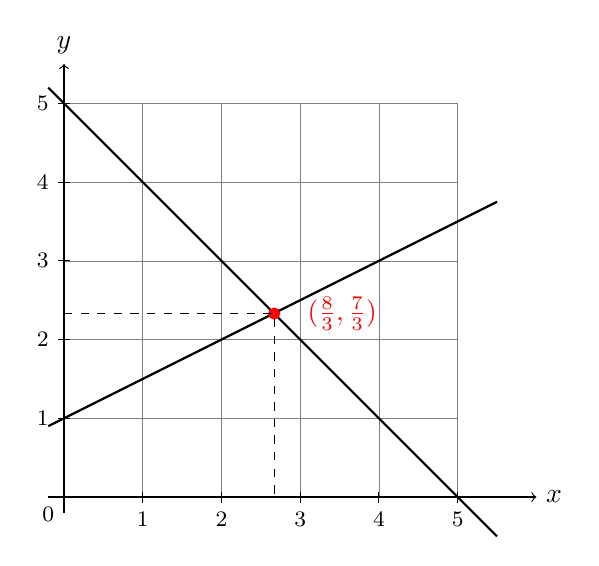
\begin{tikzpicture}[x=1cm,y=1cm]
\draw[help lines] (0,0) grid (5,5);
\draw[->] (-0.2,0) -- (6,0) node[right] {$x$};
\draw[->] (0,-0.2) -- (0,5.5) node[above] {$y$};
\foreach \x in {1,...,5}
	\draw[shift={(\x,0)}] (0pt,2pt) -- (0pt,-2pt) node[below] {\footnotesize $\x$};
\foreach \y in {1,...,5}
	\draw[shift={(0,\y)},color=black] (2pt,0pt) -- (-2pt,0pt) node[left] {\footnotesize $\y$};
\draw[thick](-0.2,5.2) -- (5.5,-0.5); % rechte 1
\draw[thick](-0.2,0.9) -- (5.5, 3.75);% rechte 2
\node [below left] at (0,0) {\footnotesize 0};
\filldraw [red] (2.67,2.33) circle (2pt) node[right=0.3cm] {$(\frac{8}{3},\frac{7}{3})$};
\draw[dashed](0,2.33) -| (2.67,0);
\end{tikzpicture}
\caption{Snijpunt van twee rechten}
    \label{fig:snijdenderechten}
\end{figure}

Er zijn verschillende methodes voor het oplossen van een stelsel van twee eerstegraadsvergelijkingen. Je herinnert je waarschijnlijk nog de \emph{substitutiemethode}\index{substitutiemethode}. Herschrijf één van beide vergelijkingen tot er staat `$\text{letter} = \ldots$'. Die letter vul je dan in (substitueren) in de andere vergelijking.

Hier zijn de vergelijkingen wel al in een eenvoudige vorm gegeven. We halen een letter uit één vergelijking: $y=-x+5$ (nogal evident, want de vergelijking staat al in de gewenste vorm). Die letter vul je in de andere vergelijking in:
\begin{align*}
y&=\frac{1}{2}x+1\\
\Leftrightarrow -x+5&=\frac{1}{2}x+1\\
\Leftrightarrow -x-\frac{1}{2}x&=-5+1\\
\Leftrightarrow -\frac{3}{2}x&=-4\\
\Leftrightarrow x&=\frac{8}{3}
\end{align*}

Deze waarde voor de onbekende $x$ vul je nu in in één van beide vergelijkingen: $y=-\frac{8}{3}+5=\frac{7}{3}$. Het snijpunt van beide rechten is dus $(\frac{8}{3},\frac{7}{3})$.

\section{Deelsgewijs lineaire functie}\label{sec:taxisprong}
\subsection{Definitie}
Soms kan een verband tussen twee grootheden voorgesteld worden door een aaneenschakeling van lineaire functies. We spreken in dit verband ook over functies met \emph{meervoudig voorschrift}\index{meervoudig voorschrift}. In algoritmes komt dit vaak voor: afhankelijk van de waarde van inputparameter(s) kunnen er verschillende berekeningen volgen (\verb+if ... then ... else ...+ constructies enz.).

Laten we even teruggrijpen naar het taxivoorbeeld (\cref{sec:taxirit}). We gingen ervan uit dat de meter `continu' doorloopt. Voor elke km, maar ook voor elke m, mm, \ldots \ loopt de prijs op. 

Dat is niet wat er in een echte taximeter gebeurt. Wie al een taxi nam, heeft gemerkt dat de meter `in sprongetjes' verhoogt. Laten we veronderstellen dat de taximeter per begonnen km een sprongetje maakt. We herhalen nog eens de getalwaarden: voor een rit in het centrum na 22 uur betaal je \euros{4,40} instapgeld en \euros{1,66} per \emph{begonnen} km. In deze veronderstelling maakt het niet uit of je nu 5,3 of 5,1 of 5,999 km rijdt. Deze drie afstanden kosten hetzelfde!

\subsection{Grafiek}
\Cref{fig:taxideels} toont de grafiek van de prijs van de taxirit in functie van de afstand in km. Aangezien de prijs gedurende een km constant blijft, bestaat de functie uit stukjes horizontale rechten. Met `open' en `gesloten' bolletjes duiden we aan welke waarde je moet kiezen in de grenspunten. Zo wijst het gesloten bolletje bij $(1;7,72)$ erop dat de functiewaarde $f(1)=7,72$.
\begin{figure}[htbp]
    \centering
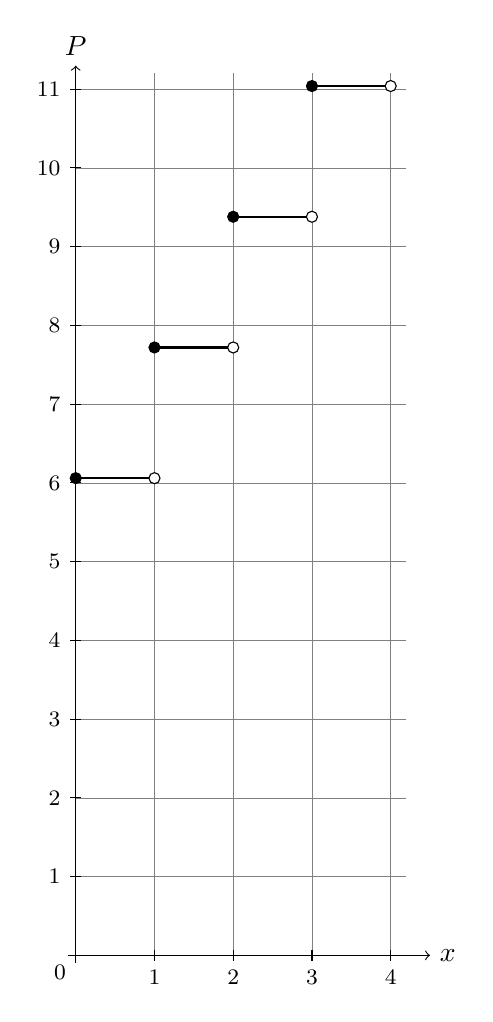
\begin{tikzpicture}[x=1cm,y=1cm]
\draw[help lines] (0,0) grid (4.2,11.2);
\draw[->] (-0.1,0) -- (4.5,0) node[right] {$x$};
\draw[->] (0,-0.1) -- (0,11.3) node[above] {$P$};
\foreach \x in {1,...,4}
	\draw[shift={(\x,0)}] (0pt,2pt) -- (0pt,-2pt) node[below] {\footnotesize $\x$};
\foreach \y in {1,...,11}
	\draw[shift={(0,\y)},color=black] (2pt,0pt) -- (-2pt,0pt) node[left] {\footnotesize $\y$};
\node [below left] at (0,0) {\footnotesize 0};
%\filldraw [red] (15,29.3) circle (2pt);
%\filldraw [red] (3,9.38) circle (2pt) node[below right] {(3;9,38)};
%\filldraw [red] (1,6.06) circle (2pt) node[below right] {(1;6,06)};
%\filldraw [red] (8,17.68) circle (2pt) node[below right] {(8;17,68)};
\draw[thick] (0,6.06) -- (1,6.06);
\draw[thick] (1,7.72) -- (2,7.72);
\draw[thick] (2,9.38) -- (3,9.38);
\draw[thick] (3,11.04) -- (4,11.04);
\filldraw[fill=black, draw=black] (0,6.06) circle (2pt);
\filldraw[fill=white, draw=black] (1,6.06) circle (2pt);
\filldraw[fill=black, draw=black] (1,7.72) circle (2pt);
\filldraw[fill=white, draw=black] (2,7.72) circle (2pt);
\filldraw[fill=black, draw=black] (2,9.38) circle (2pt);
\filldraw[fill=white, draw=black] (3,9.38) circle (2pt);
\filldraw[fill=black, draw=black] (3,11.04) circle (2pt);
\filldraw[fill=white, draw=black] (4,11.04) circle (2pt);
\end{tikzpicture}
\caption{Deelsgewijs lineaire functie}
    \label{fig:taxideels}
\end{figure}

\subsection{Voorschrift}
Er zijn verschillende manieren om een voorschrift voor deze functie te geven. De eenvoudigste, maar langste, manier bestaat erin alle verschillende gevallen te beschrijven.
\begin{equation}
P(x)=\left\{
\begin{array}{ll}
6,06 &\text{ voor } x \in [0,1[ \\
7,72 &\text{ voor } x \in [1,2[ \\
9,38 &\text{ voor } x \in [2,3[ \\
\ldots &
\end{array}
\right.
\end{equation}

Voorschrift~\eqref{eq:taxifloor} is een stuk interessanter, maar ook wel een stuk moeilijker om te vinden.
\begin{equation}\label{eq:taxifloor}
P(x)= 1,66\cdot \mathtt{floor}(x+1)+4,40
\end{equation}
De functie $\mathtt{floor}(x)$ is het grootste geheel getal niet groter dan $x$. We gebruiken hier de notatie van Scilab (en veel andere programmeertalen). In wiskunde noteert men deze \verb+floor+-functie als $\lfloor x \rfloor$.

\section{Samenvatting}
\begin{center}
  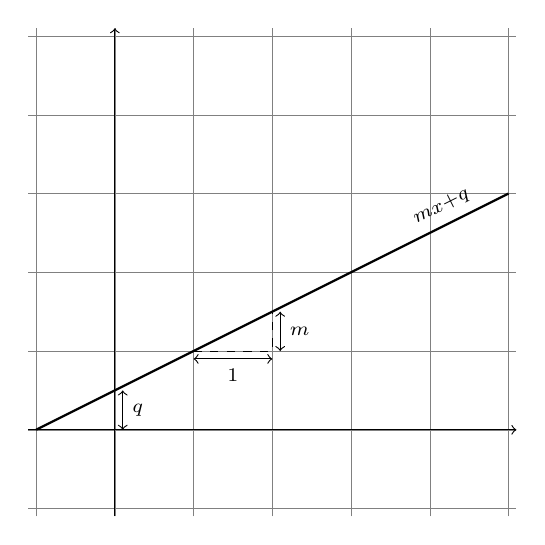
\begin{tikzpicture}
    \draw[gray,ultra thin] (-1.1,-1.1) grid (5.1,5.1);
    \draw[->] (-1.1,0) -- (5.1,0);
    \draw[->] (0,-1.1) -- (0,5.1);

    \draw[thick] (-1,0) -- (5,3) node [above,very near end,sloped] {$\scriptstyle mx+q$};

    \draw[thin,dashed] (1,1) -- (2,1) -- (2,1.5);
    \draw[<->,thin,yshift=-1mm] (1,1) -- (2,1) node [below,midway] {$\scriptstyle 1$};
    \draw[<->,thin,xshift=1mm] (2,1) -- (2,1.5) node [right,midway] {$\scriptstyle m$};
    \draw[<->,thin,xshift=1mm] (0,0) -- (0,0.5) node [right,midway] {$\scriptstyle q$};
  \end{tikzpicture}
\end{center}


\section{Oefeningen}
\begin{oef}
De rechte $r$ gaat door punten $A$ en $B$. Stel het functievoorschrift op voor $r$. Zoek het nulpunt en het snijpunt met de verticale as.
\begin{enumerate}
\item $A(2,5)$ en $B(4,-1)$
\item $A(-2,-4)$ en $B(3,-4)$
\item $A(3,-1)$ en $B(3,6)$ 
\end{enumerate}
     \begin{opl}
\begin{enumerate}
\item $f(x)=-3x+11$, nulpunt $(\frac{11}{3}, 0)$ en snijpunt met de $y$-as: $(0,11)$
\item $f(x)=-4$, dus een constante functie. Deze functie heeft geen nulpunt en het snijpunt met de $y$-as is $(0,-4)$.
\item Deze rechte heeft als vergelijking $x=3$. Het is een verticale rechte en dus geen functie. Het heeft dan ook geen zin om te spreken over nulpunt en snijpunt met de $y$-as.
\end{enumerate}
     \end{opl}
\end{oef}

\begin{oef}
Figuur~\ref{fig:rechtenoef2} toont enkele rechten in een assenkruis. Stel een vergelijking op van de rechten. Welke stellen functies voor?
\begin{figure}[htbp]
    \centering
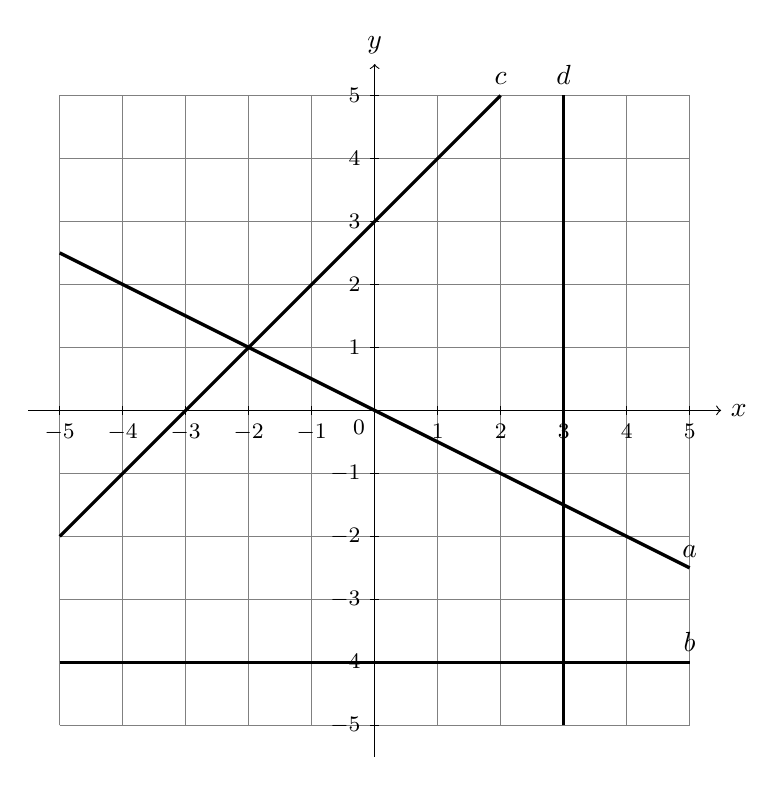
\begin{tikzpicture}[scale=0.8]
\draw[help lines] (-5,-5) grid  (5,5);
\draw[->] (-5.5,0) -- (5.5,0) node[right] {$x$};
\draw[->] (0,-5.5) -- (0,5.5) node[above] {$y$};
\foreach \x in {-5,...,-1,1,2,...,5}
	\draw[shift={(\x,0)}] (0pt,2pt) -- (0pt,-2pt) node[below] {\footnotesize $\x$};
\foreach \y in {-5,...,-1,1,2,...,5}
	\draw[shift={(0,\y)},color=black] (2pt,0pt) -- (-2pt,0pt) node[left] {\footnotesize $\y$};
\node [below left] at (0,0) {\footnotesize 0};
\draw[very thick] (-5,2.5) -- (5,-2.5) node[above] {$a$};
\draw[very thick] (-5,-4) -- (5,-4) node[above] {$b$};
\draw[very thick] (-5,-2) -- (2,5) node[above] {$c$};
\draw[very thick] (3,-5) -- (3,5) node[above] {$d$};
\end{tikzpicture}
\caption{Zoek een vergelijking voor deze rechten}
    \label{fig:rechtenoef2}
\end{figure}
\begin{opl} Enkel rechte $d$ is geen functie \\
$a\leftrightarrow y=-\frac{1}{2}x$\\
$b \leftrightarrow y=-4 $\\
$c \leftrightarrow y=x+3$\\
$d \leftrightarrow x=3$
\end{opl}
\end{oef}


\begin{oef}
Je twijfelt tussen drie verschillende tariefplannen voor telefonie. Je bent enkel geïnteresseerd in bellen (dus niet in SMS of data). Bij Proximus stelt men je het tarief `free call' voor. Echt `free' is het wel niet: je betaalt \euros{30} per maand, maar je mag wel onbeperkt bellen naar alle netwerken. Mobistar vertelt je dat hun tarief `olifant' het goedkoopste is. Je betaalt een abonnementskost van \euros{15}. Je mag dan wel een uur gratis bellen. Als je gratis uur opgebruikt is, worden je telefoongesprekken betalend tegen \euros{0,25} per minuut. Base beweert dat je nergens goedkoper belt dan met hun `simpel' herlaadkaart: geen abonnementskosten, enkel \euros{0,40} per belminuut.

Maak een figuur van de verschillende tarieven (kostprijs i.f.v. de beltijd). Duid op de figuur aan wat de goedkoopste formule is voor elke beltijd. Geef een overzichtelijk antwoord.

Stel dat je telkens voor de goedkoopste formule gaat. Hoeveel kosten dan respectievelijk 10, 100 en 1000 belminuten?
\begin{opl}
Tot een maandelijkse beltijd van 37,5 minuten is Base het goedkoopst. Tussen 37,5 en 120 minuten kan je best Mobistarklant worden. Voor wie meer belt dan twee uur per maand is Proximus het goedkoopst. 
Voor 10 belminuten kies je dus Base met een kostprijs van $10\cdot 0,40=4$ euro. Als je 100 minuten per maand belt, ben je goedkoopst bij Mobistar. Dat kost je dan \euros{25}. Wie 1000 minuten belt, hoeft niet te twijfelen: kies Proximus en dus kost het je \euros{30}.
\end{opl}
\end{oef}

\begin{oef}
De snelste supercomputer (figuur~\ref{fig:ibmBG}) in 2012 is de IBM Blue Gene Sequoia\footnote{\url{http://www.top500.org/list/2012/06/100}}.  Deze computer haalt 16324 TFlops (Teraflops). 
\begin{figure}[hbtp]
\centering
\includegraphics[width=\textwidth]{figuren/eerstegraadsfuncties/IBMBlueGene.jpg}
\caption{IBM Blue Gene supercomputer}
\label{fig:ibmBG}
\end{figure}

Eén teraflop is $10^{12}$ floating point berekeningen per seconde. Het vermogen bedraagt \SI{7,890}{\mega\watt}. Ter vergelijking: de grootste kerncentrale in Doel (4) heeft een vermogen van ongeveer \SI{1000}{\mega\watt}, wat betekent dat ongeveer 126 van dergelijke supercomputers heel de elektrische productie van Doel 4 zouden opgebruiken. Stel dat het verband tussen rekensnelheid (in TFlops) en vermogen (in \si{\mega\watt}) rechtevenredig is, wat zou dan het vermogen worden als er over afzienbare  tijd een supercomputer \num{100000} TFlops haalt (dat zijn dus \num{100000000000000000} floating point berekeningen per seconde)? Is de veronderstelling dat dit verband rechtevenredig is te verdedigen, denk je?
\begin{opl}
Eerst en vooral: de aanname van rechtevenredigheid is niet te verdedigen. Als je naar de geciteerde URL in de opgave gaat kijken, merk je dat men niet anders kan dan ook het verbruik (koeling, \ldots) in aanmerking nemen en proberen dit zo laag mogelijk te houden. Als we dan toch de evenredigheid volgen, bekomen we het antwoord dat getoond wordt in figuur~\ref{fig:rekensnelheidvermogen}.
\begin{figure}[htbp]
    \centering
\begin{tikzpicture}[x=0.08cm,y=0.15cm]
%\draw[help lines] (-5,-5) grid  (5,5);
\draw[->] (-2,0) -- (105,0) node[right] {1000 TFlops};
\draw[->] (0,-1) -- (0,52) node[above] {\si{\mega\watt}};
\foreach \x in {10,20,...,100}
	\draw[shift={(\x,0)}] (0pt,2pt) -- (0pt,-2pt) node[below] {\footnotesize $\x$};
\foreach \y in {10,20,...,50}
	\draw[shift={(0,\y)},color=black] (2pt,0pt) -- (-2pt,0pt) node[left] {\footnotesize $\y$};
\node [below left] at (0,0) {\footnotesize 0};
\draw[thick] (0,0) -- (110,53.17);
\draw[dashed] (16.324,0) |- (0,7.89);
\filldraw [red] (16.324,7.89) circle (2pt) node[below right] {$(16,324;7,89)$};
\draw[dashed] (100,0) |- (0,48.33);
\filldraw [red] (100,48.33) circle (2pt) node[below right] {$(100;48,33)$};
\end{tikzpicture}
\caption{Verband tussen vermogen en rekensnelheid}
    \label{fig:rekensnelheidvermogen}
\end{figure}
\end{opl}
\end{oef}

\begin{oef}
Een harde schijf van 500 GB kost \euros{60}. Die van 2 TB kost \euros{130}. Bij gebrek aan andere informatie gaan we ervan uit dat het verband tussen opslagcapaciteit en prijs lineair is. Hoeveel zou volgens dit verband dan een harde schijf van 1,5 TB kosten? Je mag voor de eenvoud een TB gelijk stellen aan 1000 GB (wat is de juiste waarde?). Deze techniek noemen we `lineaire interpolatie'. Wat denk je in dit verband over de prijs van een harde schijf van 5 TB?
\begin{opl}
Stel de vergelijking van de rechte door de punten $(500,60)$ en $(2000,130)$. Vul dan in deze vergelijking $x=1500$ in en je bekomt \euros{106,67}. Bij 5 TB spreken we over extrapolatie en dat is meestal vrij gevaarlijk. Hoe meer data op een harde schijf, des te groter wordt de technische uitdaging en des te kleiner worden componenten, sporen enz. Een lineair verband zal dan zeker geen goede benadering zijn!
\end{opl}
\end{oef}

\begin{oef}
In Heverlee gelden volgende tarieven voor drinkwater (exclusief 6\% BTW):
\begin{itemize}
\item Vaste vergoeding: 47 \euro/jaar 
\item Verbruik van het drinkwater:  \SI{2}{\euro\per\cubic\metre} 
\item Bijdrage voor de zuivering van drinkwater: \SI{0,9}{\euro\per\cubic\metre}  
\item Bijdrage voor de afvoer van drinkwater: \SI{1,3}{\euro\per\cubic\metre}  
\end{itemize}
\begin{enumerate}
\item Bepaal het verband tussen het te betalen bedrag aan de drinkwatermaatschappij en de verbruikte hoeveelheid water
\item Een Vlaming verbruikt gemiddeld \SI{45}{\cubic\metre}   water per jaar. Van de overheid krijgt hij \SI{15}{\cubic\metre} gratis, maar hij moet wel de bijdrage voor de zuivering en afvoer betalen. Hoe groot is de gemiddelde factuur van de Vlaming?
\end{enumerate}

\begin{opl}
\begin{enumerate}
\item Veranderlijken benoemen: $x$ is verbruikte hoeveelheid drinkwater; $B$ is het te betalen bedrag
\item $B(x)=47+(2+0,9+1,3)\cdot x=47+4,2x$
\item $B_2(x)=47+2\cdot (x-15)+(0,9+1,3)\cdot x=17+4,2\cdot x$ \\
$B_2(45)=206$. De gemiddelde Vlaming betaalt \euros{206} per jaar.
\end{enumerate}
\end{opl}
\end{oef}

\begin{oef}
In	Vlaanderen	bestaat 	je	drinkwaterfactuur	steeds	uit	twee	delen:	het	verbruik	(\SI{2}{\euro\per\cubic\metre})  	en een	bijdrage	voor	zuivering	en	afvoer	(\SI{2.2}{\euro\per\cubic\metre}).		Voor	 de	 eerste	\SI{15}{\cubic\metre} hoef	je	
niet	te	betalen	  voor	het	verbruik.	Je	moet	dan	enkel	betalen	 voor	zuivering	en	 afvoer.	

In	 Brussel	geldt	een	getrapte	tarifering: 	naargelang	je	meer	verbruikt,	 wordt	de	 prijs	per	
\SI{}{\cubic\metre} duurder.	Voor	schijf 1	(0--15 \SI{}{\cubic\metre})	betaal	je	\SI{1,88}{\euro\per\cubic\metre}.	Voor	schijf	2	(15--30 \SI{}{\cubic\metre})	
betaal	je	\SI{3,38}{\euro\per\cubic\metre}.	Voor	schijf	3	(30-60 \SI{}{\cubic\metre})	betaal	je	\SI{4}{\euro\per\cubic\metre}.	
Voor	het	water	meer dan	\SI{60}{\cubic\metre} betaal	je	zelfs	 \SI{7,33}{\euro\per\cubic\metre}.
\begin{enumerate}
\item  Definieer	in	Scilab	de	 functies	“vlaanderen” 	en	 “brussel”	die	het	te	betalen	 bedrag	
in	Vlaanderen	resp.	\ Brussel	berekent	in	functie	van	het	verbruikt	aantal \SI{}{\cubic\metre}.	Zorg	
ervoor	dat	de	input	gevalideerd	wordt!
\item Teken	beide	functies	in	één	grafiek.
\item Definieer	in	Scilab	de 	functie	“drinkwater”.	De	input	bestaat	uit	twee	parameters:	
het	aantal	verbruikte \SI{}{\cubic\metre} en	de 	woonplaats	(“vlaanderen”	of	“brussel”).	Output	is	
het	te	betalen	bedrag.
\item Definieer 	in	Scilab	de	 functie	“goedkoopste”.	De	input	is	het	aantal	verbruikte \SI{}{\cubic\metre}.	
Output	is	de 	woonplaats	én 	de	kost	met	de	goedkoopste	factuur.

\end{enumerate}

\begin{opl}
$\qquad$ \\
\begin{lstlisting}[caption={Drinkwaterverbruik in Vlaanderen en in Brussel}]
function y=vlaanderen(x)
    if x<0 then
        error("verbruik moet positief zijn")
    end
    if x<15 then
        y=2.2*x
    else
        y=2.2*x+2*(x-15)
    end
endfunction

function y=brussel(x)
    if x<0 then
        error("verbruik moet positief zijn")
    end
    if x<15 then
        y=1.88*x
    elseif x<30
        y=1.88*15+3.38*(x-15)
    elseif x<60
        y=1.88*15+3.38*15+4*(x-30)
    else
        y=1.88*15+3.38*15+4*30+7.33*(x-60)
    end
endfunction

clf
x=0:80
xgrid
plot(x,vlaanderen)
plot(x,brussel,"r")

function y=drinkwater(x,regio)
    if regio<>"vlaanderen"&regio<>"brussel" then
        error("je geeft geen geldige regio")
    end
    if regio=="vlaanderen" then
        y=vlaanderen(x)
    else
        y=brussel(x)
    end
endfunction

function [prijs,regio]=goedkoopste(x)
    if x<0 then
        error("verbruik moet positief zijn")
    end
    vlndr=vlaanderen(x)
    brsl=brussel(x)
    if vlndr<brsl then
        prijs=vlndr
        regio="vlaanderen"
    else
        prijs=brsl
        regio="brussel"
    end
endfunction


[p,r]=goedkoopste(20)
printf("Bij verbruik van 20 eenheden is regio %s het goedkoopst.\n 
		De prijs bedraag %f.",r,p)
\end{lstlisting}
\end{opl}
\end{oef}

\begin{oef}
Bij een actie op Facebook ten voordele van een goed doel belooft een bedrijf per \textit{like} een bedrag te storten
\begin{itemize}
\item voor de eerste 1000 \textit{likes} stort het bedrijf \euros 1 per \textit{like}
\item voor de 1001ste tot en met 5000ste \textit{like} stort het bedrijf \euros 0,80 per \textit{like}
\item als er nog meer \textit{likes} zijn, stort het bedrijf \euros 1,20 per \textit{like}.
\end{itemize}

\begin{enumerate}
\item 
\label{functie}
Definieer in Scilab de functie die weergeeft hoeveel geld het bedrijf moet storten in functie van het aantal \textit{likes}.
\item Teken deze functie in Scilab.
\item Het bedrijf doet uiteindelijk een storting van \euros 3656. Hoeveel \textit{likes} waren er?
\item Controleer je antwoord in Scilab met behulp van de functie gedefinieerd in \ref{functie}).
\end{enumerate}

\begin{opl}
$\qquad$ \\
\begin{lstlisting}[caption={Likes - controle}]
function y=like(x)
    if x<0 then
        error("het aantal likes moet positief zijn")
    end
    if x<=1000 then
        y=x
    elseif x<=5000
        y=1000+0.80*(x-1000)
    else
        y=1000+0.80*4000+1.20*(x-5000)
    end
endfunction

clf
x=0:7000
xgrid
plot(x,like)

like(4320)
\end{lstlisting}

Bij 4320 likes stort het bedrijf \euros 3656.
\end{opl}
\end{oef}


%%% Local Variables: 
%%% mode: latex
%%% TeX-master: "../cursusTW1"
%%% End: 


%%% Local Variables: 
%%% mode: latex
%%% TeX-master: "cursusTW1"
%%% End: 
